% IAAI/AAAI submission --- Sections 2 (System) + 3 (Main Results).
% NOTE ON TEMPLATE: the official AAAI Author Kit (aaai24.sty/aaai24.bst) is not vendored in this
% repo, so this file uses a self-contained two-column article class that approximates the AAAI
% two-column layout and compiles cleanly anywhere (tectonic / pdflatex x2, 0 undefined).
% For camera-ready, replace the preamble with \documentclass[letterpaper]{article}\usepackage{aaai24}
% and move the title/author block into \title{}/\author{}; the body below is template-agnostic.
%
% NUMBER PROVENANCE: every quantitative claim is drawn from a clone-verified CSV in paper/ on
% branch paper-writeup (CSVs imported from paper-metaclip-master / paper-aaai-rigor /
% paper-image-encoders-headadapt). Each table/figure caption names its source CSV. Unverified
% or extrapolated figures are marked [VERIFY].
\documentclass[10pt,twocolumn]{article}
\usepackage[T1]{fontenc}
\usepackage[utf8]{inputenc}
\usepackage{times}
\usepackage{amsmath,amssymb}
\usepackage{graphicx}
\usepackage{booktabs}
\usepackage{microtype}
\usepackage{tikz}
\usetikzlibrary{positioning}
\usepackage{pgfplots}
\pgfplotsset{compat=1.18}
\usepackage[hidelinks]{hyperref}
\usepackage[margin=0.75in,columnsep=0.25in]{geometry}
\setlength{\parindent}{1em}
\newcommand{\src}[1]{\footnotesize\textit{Source: #1.}}
\newcommand{\verify}[1]{\textbf{[VERIFY: #1]}}

\title{\vspace{-2em}\bfseries A Deployed 1-Bit Cross-Modal Hashing System:\\
Browser-Native Multilingual Image Search at 128 Bytes per Image}
\author{Anonymous (IAAI track)\\ \small \texttt{paper-writeup} branch}
\date{}

\begin{document}
\maketitle

\begin{abstract}
We present a deployed image--text retrieval system that compresses a frozen vision--language
encoder (SigLIP2-So400m) into \textbf{1024-bit (128-byte)} binary codes and runs search entirely
client-side via Hamming distance, with no retrieval backend. A single Matryoshka hashing head
(per-bit BatchNorm $+$ L2, sign straight-through) turns the frozen embedding into nested codes that
are independently usable at every prefix length (16--1024 bit). On COCO~5K the deployed 1-bit codes
reach \textbf{R@10 81.24 (English)} and \textbf{R@10 71.04 (Korean)}, recovering most of the
float-cosine ceiling (83.58 / 66.26) and far exceeding naive sign hashing without a head
(72.62 / 52.18). Against same-feature unsupervised hashing baselines (ITQ, LSH) the learned head
wins by a margin that widens sharply at low bit-rates (e.g. $+55$ R@10 at 64-bit). We extend the
system to 36 languages (XM3600) and to fully on-device operation: a browser query path
(int8 multilingual text encoder) and on-device photo indexing via head-adapted mobile vision
encoders that map into the same frozen code space. We report measured phone latency and the
runtime (not accuracy) constraints that force fp32-only browser inference. We do not claim to beat
float multilingual SoTA (NLLB-CLIP, XM3600 R@10 86.06); our contribution is the deployable,
backend-free, portable-index regime and an honest characterization of where it holds and where it
does not.
\end{abstract}

\section{Introduction}
Frozen-feature deep hashing---training a small head on a fixed foundation-model embedding with a
single objective---has recently been shown effective for unimodal retrieval (OrthoHash
\cite{orthohash}; HashCoder/CroVCA \cite{crovca}). Those works establish that BatchNorm-based code
balance and a single alignment loss suffice; we claim \emph{no} novelty on that point and our own
loss-composition ablations are consistent with theirs (composition and weight-tuning are inert;
BatchNorm dominates the code geometry). The open lane, and our focus, is the \textbf{cross-modal
$+$ multilingual $+$ on-device} extension: image--text retrieval, non-English text, and
browser/phone deployment, together with the failure modes that only appear there. Concretely, this
paper contributes (i) a deployed browser-native 1-bit cross-modal search system at 128~B/image
(\S2); (ii) main retrieval, multilingual, baseline, on-device-cost, and encoder-choice results,
all measured (\S3); and (iii) analysis hooks (\S4--\S7) for the main-track companion. Throughout we
prioritize measured, reproducible numbers over claims; every table cites the CSV it is computed
from.

\section{System}

\subsection{Overview}
The pipeline is a frozen encoder followed by a lightweight hashing head and client-side search
(Fig.~\ref{fig:arch}). A frozen SigLIP2-So400m encoder produces a 1152-d embedding $e$; a
\emph{NestedHashLayer} maps $e$ to a 1024-bit code. The head is a single projection
($1152\!\to\!384\!\to\!1024$) whose output is sliced to each target length $b$, then per-bit
BatchNorm and L2 normalization are applied, and the sign function (with a straight-through estimator
for training) yields the binary code $\mathbf{b}\in\{-1,+1\}^{b}$. Because shorter codes are strict
prefixes of longer ones, a single model serves every bit-rate $16\!\to\!1024$; the deployed
configuration stores the full \textbf{1024-bit = 128-byte} code per image and ranks by Hamming
distance in the client.

\begin{figure}[t]
\centering
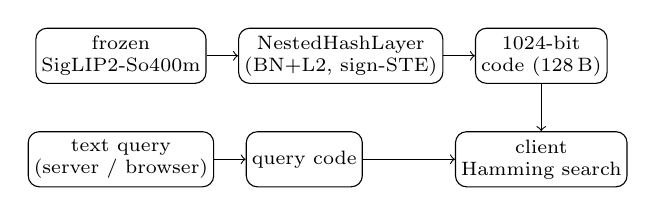
\begin{tikzpicture}[font=\scriptsize,node distance=4mm,
  box/.style={draw,rounded corners,minimum height=7mm,align=center,inner sep=2pt}]
\node[box] (enc) {frozen\\SigLIP2-So400m};
\node[box,right=of enc] (head) {NestedHashLayer\\(BN+L2, sign-STE)};
\node[box,right=of head] (code) {1024-bit\\code (128\,B)};
\node[box,below=6mm of code] (ham) {client\\Hamming search};
\draw[->] (enc) -- (head); \draw[->] (head) -- (code); \draw[->] (code) -- (ham);
\node[box,below=6mm of enc,align=center] (q) {text query\\(server / browser)};
\node[box,right=of q] (qcode) {query code};
\draw[->] (q) -- (qcode); \draw[->] (qcode) -- (ham);
\end{tikzpicture}
\caption{System architecture. Gallery codes (top) are precomputed once; queries (bottom) are
encoded by one of two text paths (\S2.2) and matched by client-side Hamming distance. No retrieval
backend.}
\label{fig:arch}
\end{figure}

\subsection{Two query paths}
The gallery is fixed (SigLIP2 image codes), but queries can be encoded two ways. The
\textbf{server path} runs the native SigLIP2 text tower, used when a (stateless) text-encoding
endpoint is available; it gives the headline numbers in \S3. The \textbf{browser path} runs a small
multilingual text encoder exported to int8 ONNX, whose output is mapped into the SigLIP2 code space
by an adapted head $\mathit{txt\_h}'$; this path is used for fully offline / private operation and
trades accuracy for backend independence (\S3.2, \S3.5). Both paths emit codes in the same 1024-bit
space, so they share one gallery index.

\subsection{On-device image indexing}
For private, on-device galleries the user's own photos must be encoded without a server. We freeze a
mobile vision encoder (e.g.\ MobileCLIP2) and train an image-side adapter $\mathit{img\_h}'$ that
maps its embedding into the \emph{same} frozen SigLIP2 1024-bit code space behind the index. The
gallery therefore stays a single frozen code space regardless of which on-device encoder produced a
given entry, and server-encoded and phone-encoded images coexist in one index. \S3.5 quantifies the
accuracy of each candidate mobile encoder.

\subsection{Deployment}
The system ships as a Progressive Web App: a portable 128-byte-per-image index, client-side Hamming
ranking, and no retrieval backend (static hosting / Cloudflare). A 50k-image index is
\textbf{6.4~MB} (1024-bit codes).\footnote{\src{paper/bits\_sweep.csv (\texttt{index\_MB\_50k})}}
Browser inference is fp32-only---not for accuracy reasons but because the WASM execution provider
cannot run int8 (\texttt{ConvInteger}) or load external-data fp16 weights (\S3.4).

\section{Main Results}

\subsection{Retrieval quality}
Table~\ref{tab:coco} reports COCO~5K retrieval for the deployed 1-bit system against the float-cosine
ceiling and against naive sign hashing of the frozen embedding (no learned head). The learned head
recovers most of the float ceiling at 1/72 of the storage (1024 bit vs.\ fp32$\times$1152) and beats
the headless naive baseline by $+8.6$ R@10 (EN) and $+18.9$ R@10 (KO). Korean even exceeds its own
float ceiling (71.04 vs.\ 66.26) because the deployed head is Korean-fine-tuned, whereas the raw
float tower is not.

\begin{table}[t]
\centering\small
\begin{tabular}{llcccc}
\toprule
lang & method & R@1 & R@5 & R@10 & mAP@10 \\
\midrule
EN & float ceiling      & 52.94 & 75.72 & 83.58 & 62.71 \\
EN & \textbf{ours 1-bit}& 43.40 & 71.16 & \textbf{81.24} & 55.15 \\
EN & naive sign         & 38.42 & 62.76 & 72.62 & 48.95 \\
\midrule
KO & float ceiling      & 31.88 & 55.32 & 66.26 & 42.15 \\
KO & \textbf{ours 1-bit}& 30.68 & 58.98 & \textbf{71.04} & 42.62 \\
KO & naive sign         & 21.74 & 42.14 & 52.18 & 30.50 \\
\bottomrule
\end{tabular}
\caption{COCO 5K, 1024-bit, lowercased eval. \src{paper/coco\_lc\_full.csv}}
\label{tab:coco}
\end{table}

\textbf{Bit-rate.} Fig.~\ref{fig:bits} sweeps code length. Quality rises steeply to 256-bit, is
near-saturated by 1024-bit (R@10 80.64, EN), and gains little beyond: 2048-bit adds only $+0.7$ for
$2\times$ storage and 4096-bit does not improve further. 1024-bit (128~B) is the deployed sweet spot.

\begin{figure}[t]
\centering
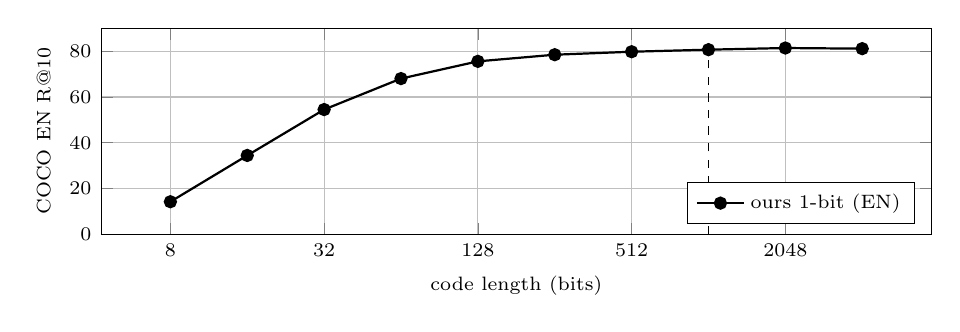
\begin{tikzpicture}
\begin{axis}[width=\columnwidth,height=4.2cm,xmode=log,log basis x=2,
  xlabel={code length (bits)},ylabel={COCO EN R@10},
  xtick={8,32,128,512,2048},xticklabels={8,32,128,512,2048},
  ymin=0,ymax=90,grid=both,tick label style={font=\scriptsize},
  label style={font=\scriptsize},legend style={font=\scriptsize,at={(0.98,0.05)},anchor=south east}]
\addplot[mark=*,thick] coordinates
 {(8,14.26)(16,34.46)(32,54.5)(64,68.02)(128,75.54)(256,78.44)(512,79.74)(1024,80.64)(2048,81.36)(4096,81.08)};
\addlegendentry{ours 1-bit (EN)}
\draw[dashed] (axis cs:1024,0) -- (axis cs:1024,80.64);
\end{axis}
\end{tikzpicture}
\caption{Bit-rate sweep, COCO EN, lowercased. \src{paper/bits\_extreme\_lc.csv (lower rows)}}
\label{fig:bits}
\end{figure}

\subsection{Multilingual}
On XM3600 (36 languages, text$\to$image), the deployed server head averages \textbf{R@10 70.30},
versus a float ceiling of 74.46; the fully offline browser encoder (MiniLM-L12) averages 53.92
(Table~\ref{tab:multiling}). The server path leads on average, but on four low-resource, non-Latin
languages---Hindi, Telugu, Thai, Maori---the offline multilingual encoder \emph{beats} the SigLIP2
server path (e.g.\ Hindi 52.36 offline vs.\ 43.38 server), and on five it beats even the float
ceiling. The multilingual text tower, not the binarization, is the bottleneck on those scripts.

\begin{table}[t]
\centering\small
\begin{tabular}{lcc}
\toprule
configuration & XM3600 avg-36 R@10 & deployable \\
\midrule
float ceiling (SigLIP2)        & 74.46 & no \\
\textbf{server (ours, 1-bit)}  & \textbf{70.30} & no \\
offline MiniLM (ours, 1-bit)   & 53.92 & \textbf{browser} \\
\bottomrule
\end{tabular}
\caption{XM3600 36-language average. Offline beats server on \{hi, te, th, mi\}.
\src{paper/multiling\_server\_lc.csv, paper/master\_table.csv}}
\label{tab:multiling}
\end{table}

\subsection{Baselines}
Table~\ref{tab:baselines} compares the learned head against ITQ and LSH applied to the
\emph{same} frozen SigLIP2 features, in a common evaluation harness (text$\to$image). The learned
head wins at every bit-rate and the margin widens dramatically as bits shrink: at 1024-bit it leads
ITQ by $+8.7$ R@10, but at 64-bit by $+55$ and at 256-bit by $+29$---data-driven binarization
matters most exactly where storage is tightest. We do \emph{not} beat float multilingual SoTA:
NLLB-CLIP's float ceiling reaches XM3600 R@10 86.06,\footnote{\src{paper/master\_table.csv,
paper/nllb\_hashing.csv}} and as a server float model it is a different operating point; our claim
is the 1-bit, 128-byte, backend-free regime, where a 1-bit NLLB-CLIP head reaches only 51.45.

\begin{table}[t]
\centering\small
\begin{tabular}{lccc}
\toprule
bits & ours 1-bit & ITQ & LSH \\
\midrule
64   & \textbf{66.86} & 11.92 & 5.64 \\
256  & \textbf{77.48} & 48.52 & 22.88 \\
1024 & \textbf{79.92} & 71.26 & 59.36 \\
\bottomrule
\end{tabular}
\caption{COCO 5K T2I R@10, same frozen features, common harness.
\src{paper/rigor\_map\_bit.csv (ours), paper/rigor\_baselines.csv (ITQ/LSH)}}
\label{tab:baselines}
\end{table}

\subsection{On-device cost}
Table~\ref{tab:cost} collects measured deployment costs. \emph{Search} is interactive entirely in
the client: a numpy Hamming brute-force over a 5K$\times$1024-bit index (0.64~MB) takes 1.73~ms per
query and matches exact recall to within 0.8\%; an exact binary FAISS index is 0.033~ms/query.
\emph{Storage} is 128~B/image (6.4~MB for 50k). \emph{On-device image encoding} (the indexing cost)
is bounded by the browser runtime: WASM-fp32 per-photo latency is 263~ms (MobileCLIP2-S0) to 1066~ms
(S2) on an emulated Pixel~7. Crucially, fp32-only is forced by operator/format support, not
precision: int8 codes are numerically near-lossless (EN R@10 81.04 vs.\ 81.24; KO 70.52 vs.\ 71.04),
but the WASM provider lacks \texttt{ConvInteger}.

\begin{table}[t]
\centering\small
\resizebox{\columnwidth}{!}{%
\begin{tabular}{lll}
\toprule
component & cost & source \\
\midrule
search (client numpy) & 1.73 ms/query & rigor\_faiss\_bench \\
search (FAISS exact)   & 0.033 ms/query & rigor\_faiss\_bench \\
storage                & 128 B/image (6.4 MB/50k) & bits\_sweep \\
img encode S0 (WASM)   & 263 ms/photo & PILLAR1\_DEPLOY \\
img encode S2 (WASM)   & 1066 ms/photo & PILLAR1\_DEPLOY \\
int8 code accuracy     & 81.04/70.52 R@10 & precision\_lc \\
\bottomrule
\end{tabular}}
\caption{Measured on-device costs. Search index is 5K images; a 50k extrapolation
(\,$\approx$0.33/15 ms\,) is \protect\verify{not directly benchmarked at 50k}. Browser text-query
latency \protect\verify{not measured in repo CSVs}.}
\label{tab:cost}
\end{table}

\subsection{Encoder choice for on-device indexing}
Table~\ref{tab:encoders} sweeps ten candidate on-device image encoders, each head-adapted into the
frozen SigLIP2 code space; the anchor (full SigLIP2 image tower) is R@10 81.24. The dominant factor
is vision--language pretraining, not parameter count: MobileCLIP2-S0 (11.4~M, VL-pretrained) reaches
70.52, beating the larger image-only-SSL DINOv2-base (86.6~M, 65.0). MobileCLIP2-S2 (35.8~M) is the
practical sweet spot at 76.18---near the 92.9~M SigLIP2-base (77.98) at a fraction of the size and
latency (Fig.~\ref{fig:enc}).

\begin{figure}[t]
\centering
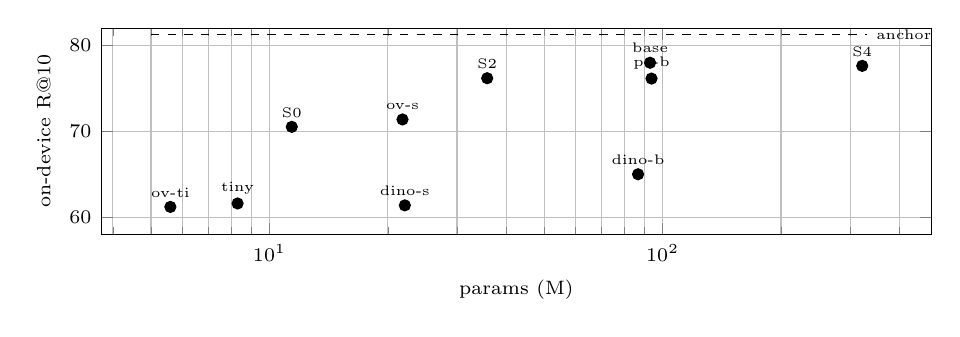
\begin{tikzpicture}
\begin{axis}[width=\columnwidth,height=4.2cm,xmode=log,
  xlabel={params (M)},ylabel={on-device R@10},
  ymin=58,ymax=82,grid=both,tick label style={font=\scriptsize},label style={font=\scriptsize},
  nodes near coords,every node near coord/.style={font=\tiny},point meta=explicit symbolic]
\addplot[only marks,mark=*] coordinates {
 (11.4,70.52)[S0] (35.8,76.18)[S2] (321.8,77.62)[S4]
 (92.9,77.98)[base] (86.6,65.0)[dino-b] (22.1,61.38)[dino-s]
 (5.6,61.2)[ov-ti] (21.8,71.38)[ov-s] (93.7,76.14)[pe-b] (8.3,61.6)[tiny] };
\draw[dashed] (axis cs:5,81.24) -- (axis cs:330,81.24) node[right,font=\tiny]{anchor};
\end{axis}
\end{tikzpicture}
\caption{On-device image-indexing R@10 vs.\ encoder size (EN, server-side eval). VL-pretrained small
encoders beat larger image-only-SSL ones. \src{paper/image\_encoders\_headadapt.csv}}
\label{fig:enc}
\end{figure}

\begin{table}[t]
\centering\small
\begin{tabular}{lcc}
\toprule
encoder & params (M) & R@10 \\
\midrule
SigLIP2 image (anchor) & 707.8 & 81.24 \\
SigLIP2-base           & 92.9  & 77.98 \\
MobileCLIP2-S4         & 321.8 & 77.62 \\
MobileCLIP2-S2         & 35.8  & 76.18 \\
PE-Core-B16            & 93.7  & 76.14 \\
OpenVision-S16         & 21.8  & 71.38 \\
MobileCLIP2-S0         & 11.4  & 70.52 \\
DINOv2-base            & 86.6  & 65.0  \\
TinyCLIP-8M            & 8.3   & 61.6  \\
DINOv2-small           & 22.1  & 61.38 \\
OpenVision-Ti16        & 5.6   & 61.2  \\
\bottomrule
\end{tabular}
\caption{On-device encoder sweep (COCO EN R@10, head-adapted). \src{paper/image\_encoders\_headadapt.csv}}
\label{tab:encoders}
\end{table}

\section{Analysis: Why Binarization, Not Dimension, Is the Cost}
\emph{(Main-track companion --- to be written.)} Continuous dimension reduction is nearly free while
sign binarization is the dominant low-bit loss; recoverable in part by asymmetric search.

\section{Failure Modes Unique to Cross-Modal/Multilingual Hashing}
\emph{(To be written.)} Distillation's cross-modal binary-parity collapse; non-Latin script
degradation traced to the text tower.

\section{Related Work}
\emph{(To be written.)} OrthoHash \cite{orthohash} and HashCoder/CroVCA \cite{crovca} establish
single-loss frozen-feature hashing (BatchNorm balance); we extend to cross-modal, multilingual, and
on-device, and characterize the failure modes there. \verify{phrase HashCoder cross-modal scope
without quoting an unverified future-work sentence.}

\section{Conclusion}
\emph{(To be written.)} A deployed, backend-free 1-bit multilingual image search system; honest
scope (does not beat float multilingual SoTA), measured costs, and reproducible numbers.

\begin{thebibliography}{9}
\bibitem{orthohash} Hoe, J.T.; et al. One Loss for All: Deep Hashing with a Single Cosine Similarity
based Learning Objective. \emph{NeurIPS}, 2021.
\bibitem{crovca} Cross-View Code Alignment (HashCoder / CroVCA). arXiv:2510.27584, 2025.
\end{thebibliography}

\end{document}
